%\begin{enumerate}[1.]
%\numberwithin{equation}{\thesubsection.enumi}

%\begin{enumerate}[label=\arabic*.,ref=\thesection]
\renewcommand{\theequation}{\theenumi}
\begin{enumerate}[label=\arabic*.,ref=\thesubsection.\theenumi]
%\begin{enumerate}[label=\arabic*.,ref=\thesubsection.\theenumi]
%\numberwithin{equation}{subsection}

%\begin{enumerate}[label=\arabic*.,ref=\thesubsection.\theenumi]
%\begin{enumerate}[label=\thesection.\arabic*,ref=\thesection.\theenumi]

%\numberwithin{equation}{enumi}
\item Find the distance between 
\begin{align}
\vec{P} = \myvec{-2\\4}, \vec{Q} = \myvec{3\\-5}
\end{align}
%Mark on a diagram the points $\myvec{-2,4}, \myvec{3,-5}$ and find the distance between them.
\solution
Two point are P($x_{1},y_{1}$) and Q($x_{2},y_{2}$). The distance between both points is d.\\
\begin{align}
    \vec{Z} = \vec{P} - \vec{Q}  
\end{align}   
\vspace{0.5 cm}
Then the distance between P and Q is given by:

\begin{align}
   d = \norm{\vec{Z}}
\end{align}
\begin{align}
   d = \norm{\vec{P} - \vec{Q}} 
\end{align}

So, the distance between given points P and Q is:
\begin{align}
   d = \sqrt{(-2-3)^2 + (4-(-5))^2}    
\end{align}
\begin{align}
   d = \sqrt{25+81}    
\end{align}
\begin{align}
   d = \sqrt{106}    
\end{align}
So, the distance between P(-2,4) and Q(3,-5) is :
\begin{align}
   d = \sqrt{106}
\end{align}

\begin{figure}[t]
    \centering
    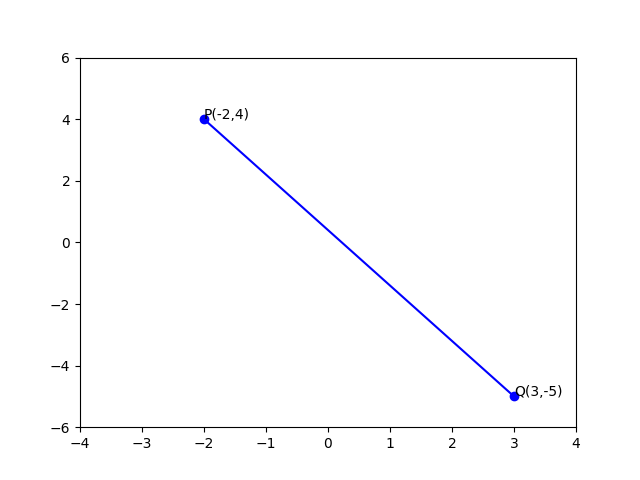
\includegraphics[width = \columnwidth]{./solutions/1/1/1/AI_assignment_1.png}
    \caption{Line between two points}
    \label{eq:solutions/1/1/1/fig:Line between two points}
\end{figure}



%
\item
Find the length of $PQ$ for
\begin{enumerate}
\item $\vec{P}=\myvec{-1\\1}$ and $\vec{Q}=\myvec{2\\-1}$;
\item $\vec{P}=\myvec{4\\3}$ and $\vec{Q}=\myvec{-2\\2}$;
\item $\vec{P}=\myvec{a\\b}$ and $\vec{Q}=\myvec{-b\\a}$.
\end{enumerate}
\solution
\begin{enumerate}
	\item The distance between $\vec{P}$ and $\vec{Q}$ is given
by:
\begin{align}
  d &= \norm{\vec{P} - \vec{Q}} \\
   &= \sqrt{(-1-2)^{2} + (1+1)^{2}}\\
   &= \sqrt{9+4}
  = 3.6055
\end{align}
	\item  
\begin{align}
    \vec{R}&=\myvec{4\\3}-\myvec{-2\\2}\\
 &=\myvec{6\\1}\label{rams/1/1/2/2eq2}
\end{align}    
The desired distance between $\vec{P}$ and $\vec{Q}$ is 
%
\begin{align}
    d&=\norm{\vec{P}-\vec{Q}}\label{rams/1/1/2/2eq1}
\end{align}
%
From \eqref{rams/1/1/2/2eq1} and \eqref{rams/1/1/2/2eq2}
\begin{align}
    d&=\norm{\vec{R}}\\
    &=\sqrt{37}
\end{align}
\end{enumerate}

\item Using direction vectors, show that  $\myvec{2\\1}, \myvec{4\\7}, \myvec{5\\4}$ and $\myvec{1\\4}$ are the vertices of a parallelogram.
\solution
Two lines are parallel if their respective directional vectors are in the same ratio.\\
Let the points be denoted by:
 \begin{align}
     \vec{A}= \myvec{2 \\1}\\
     \vec{B}= \myvec{5 \\4}\\
     \vec{C}=\myvec{4 \\7}\\
      \vec{D}=\myvec{1 \\4 }
 \end{align}
 The directional vector of $\vec{AB}$ is
\begin{align}
\myvec{2-5\\1-4}=\myvec{-3 \\-3}
\end{align}
The directional vector of $\vec{BC}$ is
\begin{align}
\myvec{5-4\\4-7}=\myvec{1 \\-3}
\end{align}
The directional vector of $\vec{CD}$ is
\begin{align}
\myvec{4-1\\7-4}=\myvec{3 \\3}
\end{align}
The directional vector of $\vec{AD}$ is
\begin{align}
\myvec{2-1\\1-4}=\myvec{1 \\-3}
\end{align}
The directional vector of $\vec{AC}$ is
\begin{align}
\myvec{2-4\\1-7}=\myvec{-2 \\-6}
\end{align}
Since the directional vectors of $\vec{AB}$ and $\vec{CD}$ are in the same ratio, so $\vec{AB}$ and $\vec{CD}$ are parallel and also opposite to each other.\\
Similarly, the directional vectors of $\vec{BC}$ and $\vec{AD}$ are in the same ratio,hence $\vec{BC}$ and $\vec{AD}$ are parallel and opposite.\\ 
Since the two pairs of opposite sides are parallel, the given points are the vertices of the parallelogram.\\

Moreover the sum of the directional vectors of $\vec{AB}$ and $\vec{BC}$ \\
  
\myvec{-3\\-3}+\myvec{1 \\-3}= \myvec{-3+1 \\-3-3}=\myvec{-2 \\-6}\\

Thus $\vec{AB}$ $+$ $\vec{BC}$= $\vec{AC}$, which satisfy
parallelogram law of vector addition i.e vector
sum of two adjacent side of a parallelogram is the
diagonal vector of the parallelogram.  See Fig.     \ref{eq:solutions/1/1/3/myfig:1}

\begin{figure}[!]
 \begin{center}
  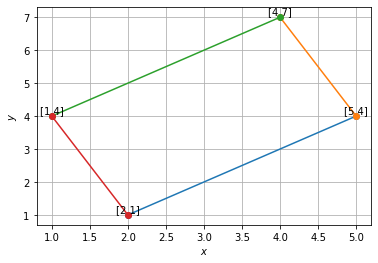
\includegraphics[width=\columnwidth]{solutions/1/1/3/assignment2_fig.png}
    \caption{This is the 2D diagram of the parallelogram with the given vertices}
    \label{eq:solutions/1/1/3/myfig:1}
    \end{center}
\end{figure}

\item Using Baudhayana's theorem, show that the points $\myvec{-3\\-4}, \myvec{2\\6}$ and $\myvec{-6\\10}$  are the vertices of a right-angled
traingle.  Repeat using orthogonality.
\solution
\begin{figure}[h!]

\centering
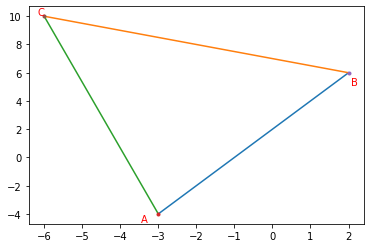
\includegraphics[width=0.5\textwidth]{solutions/1/1/4/Figure_1}
\caption{Right Angled Triangle}
\label{eq:solutions/1/1/4/fig:triangle}
\end{figure}
Say there exists two points $\textbf{P}(x_1, y_1)$ and $\textbf{Q}(x_2, y_2)$. The distance between the points is:
% Equation of y axis is 
\begin{align}
    \textbf{Z = P - Q}
\end{align}
Distance between \textbf{P} and \textbf{Q} is given by 
% For   $\Vec{
% 1 & -2 \\
% }x = 4$ (at y axis meet)
\begin{align}
||\textbf{Z}|| = \norm{\textbf{P-Q}}
\end{align}
% \begin{align}
% d = 
% \end{align}
Let $\textbf{P} = (-3, -4)$, $\textbf{Q} = (2, 6)$ and $\textbf{R} = (-6, 10)$.
\begin{enumerate}
    \item Distance between \textbf{P} and \textbf{Q} is 
\begin{align}
\norm{\textbf{P-Q}} = \sqrt{(-3-2)^2+(-4-6)^2}
=\sqrt{125}
\end{align}
\item Distance between \textbf{Q} and \textbf{R} is 
\begin{align}
\norm{\textbf{Q-R}} = \sqrt{(2-(-6))^2+(6-10)^2}
=\sqrt{80}
\end{align}
\item Distance between \textbf{P} and \textbf{R} is 
\begin{align}
\norm{\textbf{P-R}} = \sqrt{(-3-(-6))^2+(-4-10)^2}
=\sqrt{205}
\end{align}
\end{enumerate}
Here, the largest distance is $\sqrt{205}$. To be vertices of a right angled triangle, we should have 
\begin{align}
  \norm{\textbf{P-Q}}^2 + \norm{\textbf{Q-R}}^2 = \norm{\textbf{R-P}}^2
\end{align}
\begin{align}
  (\sqrt{205})^2 = (\sqrt{125})^2 + (\sqrt{80})^2
\end{align}
\begin{align}
  205 = 205
\end{align}
So, the condition is satisfied. 
So, using Baudhayana's theorem, it is proved that 3 points given are vertices of a right angled triangle. 
Now, for orthogonality, 
\begin{align}
    (\vec{P-Q})^T(\vec{Q-R}) = 0
\end{align}
We have 
\begin{enumerate}
    
    \item \begin{align}
    \vec{P-Q} = (2-(-3), 6-(-4))
\\
\vec{P-Q} = \myvec{
5\\
10 
}
\end{align}
    \item \begin{align}
    \vec{Q-R} = (2-(-6), 6-10)
\\
\vec{Q-R} = \myvec{
8\\
-4 
}
\end{align}
\item \begin{align}
    \vec{P-R} = (-3-(-6), -4-10)
\\
\vec{P-R} = \myvec{
3\\
-14 
}
\end{align}
\end{enumerate}
% We have 
% % \overrightarrow{\text {PQ}}
% \begin{align}
% \textbf{P}
% \\
%          \textbf{X}=(2-(-3), 6-(-4))
%  \\\textbf{X}= \myvec{
% 5\\
% 10 
% }
% \end{align}
% \overrightarrow{\text {QR}}
% Assuming Y is the vector, connecting Q and R. 
% \begin{align}
% \textbf{Y} = $$Q-R$$
% \\
%          \textbf{Y}=(2-(-6), 6-10)
%  \\\textbf{Y}= \myvec{
% 8\\
% -4 
% }
% \end{align}
% Assuming Z is the vector connecting P and R. 
% \begin{align}
% \textbf{Z} = $$P-R$$
% \\
%          \textbf{Z}=(-3-(-6), -4-10)
%  \\\textbf{Z}= \myvec{
% 3\\
% -14 
% }
% \end{align}
For orthogonality, product of transpose of one point and other must be 0. 
Here, checking for 
\begin{align}
    \myvec{
5\\
10 
}^T\myvec{ 8\\
-4
} =  \myvec{
5\\
10
}^T \myvec{
8 \\ -4
}=0
\end{align}
Hence, using orthogonality, it is proved that the points form a right angled triangle. 

%\section{figure}

Figure \ref{eq:solutions/1/1/4/fig:triangle} Right anlged triangle where A=P and B=Q and C=R



\item Plot the points $\myvec{0\\2},\myvec{1\\1},\myvec{4\\4}\text{ and }\myvec{3\\5}$ and prove that they are the vertices of a rectangle.
\item Show that $\vec{B}=\myvec{-2\\-2},\vec{A}=\myvec{-1\\2}\text{ and }\vec{C}=\myvec{3\\1}$ are the vertices of an isosceles triangle.
\\
\solution

Define a matrix $\vec{M}$ such that,
\begin{align}
    \vec{M} &= \myvec{\vec{B-A} & \vec{C-A}}^T\\
    \vec{M} &= \myvec{-1 & -4\\4 & -1}
\end{align}
Using matrix transformation,
\begin{align}
    \vec{M} = \myvec{-1 & -4\\4 & -1}\xleftrightarrow{R_1\leftarrow -R_1 - \frac{R_2}{4}} \myvec{0 & \frac{17}{4}\\4 & -1}\\
    \implies rank(\vec{M}) = 2
\end{align}
Since the rank of matrix $\vec{M}$ is 2, the points form a triangle.
\begin{align}
    AB^2 &= \brak{\vec{A} - \vec{B}}^T\brak{\vec{A} - \vec{B}}\\
    &= 17\\
    BC^2 &= \brak{\vec{B} - \vec{C}}^T\brak{\vec{B} - \vec{C}}\\
    &= 34
    \\
    CA^2 &= \brak{\vec{C} - \vec{A}}^T\brak{\vec{C} - \vec{A}}\\
    &= 17
    \\
    \implies AB &= AC
\end{align}
Hence, the triangle is isosceles.  See Fig.     \ref{rams/1/1/6fig:plot}
\begin{figure}[htp]
    \centering
    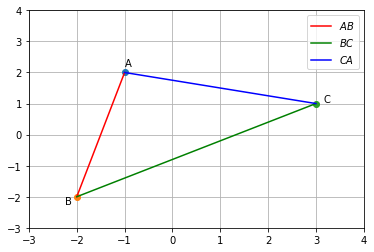
\includegraphics[width=\columnwidth]{solutions/1/1/6/Figures/Fig1.png}
    \caption{Plot of the given points}
    \label{rams/1/1/6fig:plot}
\end{figure}


\item In the last question, find the distance of the vertex $\vec{A}$ of the triangle from the middle point of the base $BC$.
\\
\solution

From the given information, 
\begin{align}
    a^2 &= (\vec{B} - \vec{C})^T(\vec{B} - \vec{C}) \\
    &= 34\\
    c^2 &= (\vec{A} - \vec{B})^T(\vec{A} - \vec{B}) \\
    &= 17\\
    b^2 &= (\vec{C} - \vec{A})^T(\vec{C} - \vec{A}) \\
    &= 17\\
    \implies AB = AC
\end{align}
Thus, the required distance is AD where
\begin{align}
     \vec{D}= \frac{\vec{B} + \vec{C}}{2} = \myvec{\frac{-1}{2}\\ \frac{-1}{2}}
\end{align}
\begin{figure}[htp]
    \centering
    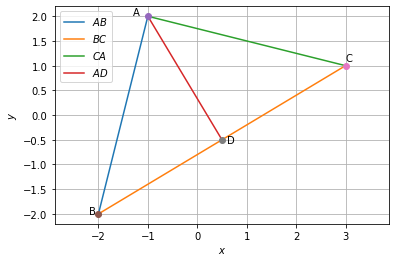
\includegraphics[width=\columnwidth]{solutions/1/1/7/figure/Assignment_1.png}
    \caption{plot}
    \label{rams/1/1/7/fig:my_label}
\end{figure}
and 
\begin{align}
    AD &= \norm{\vec{A} - \vec{D}} \\    
    &= \frac{\sqrt{34}}{2}
\end{align}



\item Prove that the points $\myvec{-1\\0}$, $\myvec{0\\3}$, $\myvec{3\\2}$ and $\myvec{2\\-1}$ are the vertices of a square.
\item Prove that the points $\vec{A}=\myvec{-1\\0}$, $\vec{B}=\myvec{3\\1}$, $\vec{C}=\myvec{2\\2}$  and $\vec{D}=\myvec{-2\\1}$ are the vertices of a parallelogram.  Find $\vec{E},\vec{F},\vec{G},\vec{H}$, the mid points of $AB, BC, CD, AD$ respectively.  Show that EG and FH bisect each other.
\\
\solution
\begin{align}
    \vec{A} - \vec{B} &=  \myvec{-4\\-1}
    \label{AB}
    \\
    &= -\brak{\vec{C} - \vec{D}}
    \\
\vec{B} - \vec{C} &=
    \myvec{1\\-1}
    \vec{A} - \vec{D} 
    \label{AD}
    \\
    \implies AB \parallel CD,  & BC \parallel AD 
\end{align}
Hence, $ABCD$ is a parallelogram.  Also, 
%
\begin{align}
    \vec{E} &= \frac{\vec{A} + \vec{B}}{2} =   \myvec{1\\\frac{1}{2}}
    \\
    \vec{F} &= \frac{\vec{B} + \vec{C}}{2} =   \myvec{\frac{5}{2}\\\frac{3}{2}}
    \\
    \vec{G} &= \frac{\vec{C} + \vec{D}}{2} = \myvec{0\\\frac{3}{2}}
\\
\vec{H} &= \frac{\vec{A} + \vec{D}}{2} =   \myvec{\frac{-3}{2}\\\frac{1}{2}}
\end{align}\\
and 
\begin{align}
 \frac{\vec{E} + \vec{G}}{2} &=   \myvec{\frac{1}{2}\\1}\\
 & = \frac{\vec{F} + \vec{H}}{2} 
\end{align}
See Fig. \ref{fig;ramsey/1/1/9}.
 \begin{figure}[!ht]
 \centering
 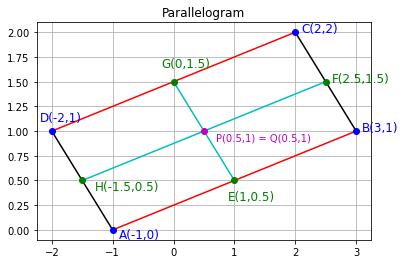
\includegraphics[width=\columnwidth]{solutions/1/1/9/parallelogram.png}
 \caption{}
 \label{fig;ramsey/1/1/9}
 \end{figure}



\item Prove that the points $\myvec{21\\-2}$, $\myvec{15\\10}$, $\myvec{-5\\0}$  and $\myvec{1\\-12}$ are the vertices of a rectangle, and find the
coordinates of its centre.
\\
\solution
Let    
    \begin{align}    
    \vec{A} = \myvec{21\\-2},
    \vec{B} = \myvec{15\\10},
    \vec{C} = \myvec{-5\\0},
    \vec{D} = \myvec{1\\-12}\label{rams/1/1/10/eq 2.0.1}
    \end{align}
    Then, 
    \begin{align}
        \vec{A} - \vec{B} *= \myvec{6 \\ -12}
    \\
    \vec{B} - \vec{C}     &= \myvec{20 \\ 10}
    \\
    \vec{C} - \vec{D}      & = \myvec{-6 \\ 12}
    \\
    \vec{D} - \vec{A}    & = \myvec{-20 \\ -10}
    \end{align}
    Since the directional vectors of $\vec{AB}$ and $\vec{CD}$
    are in the same ratio, so  $\vec{AB}$ and $\vec{CD}$ are
    parallel and also opposite to each other.
    Similarly, $\vec{BC}$ and $\vec{DA}$ are parallel and opposite.
    %
    Hence ABCD is a parallelogram.  Also, 
    \begin{align}
     (\vec{\vec{B} - \vec{A}})^\top(\vec{\vec{C} - \vec{B}}) 
        &= \myvec{-6 & 12} \myvec{-20 \\ -10}\\
        &= 0
    \end{align}
    Therefore, one of the angle is right angle and ABCD is a rectangle.
    The center
    \begin{align}
        \vec{O} &= \frac{\vec{A}+ \vec{C}}{2}\\
        &= \myvec{8 \\ -1}
    \end{align}
    This is verified in Fig. \ref{rams/1/1/10/fig:my_label}.
    \begin{figure}[htp]
        \centering
        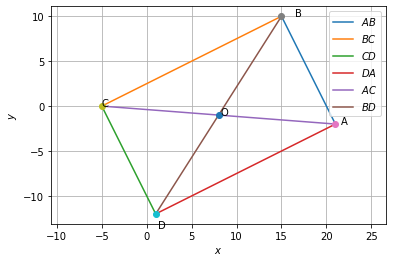
\includegraphics[width=\columnwidth]{solutions/1/1/10/Figure/AS1.png}
        \caption{plot}
        \label{rams/1/1/10/fig:my_label}
    \end{figure}
%
\item Find the lengths of the medians of the triangle whose vertices are at the points $\myvec{1\\2}$, $\myvec{0\\3}$ and $\myvec{-1\\-2}$.
\item Find the coordinates of the points that divide the line joining the points $\myvec{-35\\-20}$ and $\myvec{5\\-10}$ into four equal parts.
\item Find the coordinates of the points of trisection of the line joining the points $\myvec{-5\\5}$ and $\myvec{25\\10}$.
\item Prove that the middle point of the line joining the points $\myvec{-5\\12}$ and $\myvec{9\\-2}$ is a point of trisection of the line
joining the points $\myvec{-8\\-5}$ and $\myvec{7\\10}$.
\\
\solution
% % Let 
% % \begin{align}
% %     \vec{A} = \myvec{-5\\12}, \vec{B{} = \myvec{9\\-2}$
% % \end{align}
% % Then 
% % \begin{align}
% %     \vec{C}&=\frac{{B}+{A}}{1+1}=\frac{{B}+{A}}{2}\\
% %     &= \frac{\myvec{9\\-2}+\myvec{-5\\12}}{2}\\
% %     \implies {C}&= \myvec{2\\5}
% % \end{align}
% % And now we have to find the ratio in which C divides the line
% % joining the points P = $\myvec{-8\\-5}$ and Q = $\myvec{7\\10}$. Let the ratio is $k:1$,
% % Then,
% % \begin{align}
% %     \implies {C}&=\frac{k{Q}+{P}}{k+1}\\
% %     \myvec{2\\5} &= \frac{{k{\myvec{7\\10}+\myvec{-8\\-5}}}}{k+1}\\
% %     \myvec{2\\5}&=\frac{1}{k+1} \myvec{7k-8\\10k-5}\\
% %     \implies k &= 2
% % \end{align}
% % As $k=2$, That implies C divides the line
% % joining the points P = $\myvec{-8\\-5}$ and Q = $\myvec{7\\10}$ in the ratio $2:1$.

% % $\therefore$ C is point of trisection of line joining P and Q.

% \begin{figure}[htp]
%     \centering
%     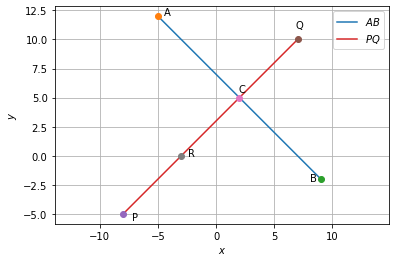
\includegraphics[width=\columnwidth]{solutions/1/1/14/a_1.png}
%     \caption{}
%     \label{fig:ramsey/1/1/14/}
% \end{figure}

% $\therefore$ The middle point of the line joining the points $\myvec{-5\\12}$ and $\myvec{9\\-2}$ is a point of trisection of the line
% joining the points $\myvec{-8\\-5}$ and $\myvec{7\\10}$.


\item The points $\myvec{8\\5}$, $\myvec{-7\\-5}$ and $\myvec{-5\\5}$ are three of the vertices of a parallelogram.  Find the coordinates of
the remaining vertex which is to be taken as opposite to $\myvec{-7\\-5}$.
\item The point $\myvec{2\\6}$ is the intesection of the diagonals of a parallelogram two of whose vertices are at the points $\myvec{7\\16}$ and $\myvec{10\\2}$.
Find the coordinates of the remaining vertices.
\item Find the area of the triangle whose vertices are the points $\myvec{2\\3}$, $\myvec{-4\\7}$ and $\myvec{5\\-2}$.  
\item Find the coordinates of  points which divide the join of $\myvec{2\\3}$, $\myvec{-4\\5}$ externally in the ratio $2:3$, and also
externally in the ratio $3:2$.
\item Prove the centroid of $\triangle ABC$ is
\begin{equation}
\vec{O}=\frac{\vec{A}+\vec{B}+\vec{C}}{3}
\end{equation}

\end{enumerate}
%\bibliography{IEEEabrv,gvv_opt}

%\input{./chapters/chapter2} 
%%
%\newpage
%\section{$M$-ary Modulation}
%\input{./chapters/chapter3} 
%
%\newpage
%\section{BER in Rayleigh Flat Slowly Fading Channels}
	%\input{./chapters/chapter4} 




